\documentclass{article}

\usepackage[utf8]{inputenc}
\usepackage{mathtools, amssymb}
\usepackage{caption}
\usepackage{subcaption}
\usepackage{graphicx}
\usepackage{booktabs}

\graphicspath{ {./images/} }

\DeclarePairedDelimiter{\abs}{\lvert}{\rvert}
\DeclarePairedDelimiter{\norm}{\lVert}{\rVert}

\title{Monocular Scale}
\author{alex.kreimer}
\date{May 2016}

\begin{document}

\maketitle

\section{The dataset}

We train and test on the KITTI dataset. There are 11 sequences with
the vehicle path ground truth and 10 more sequences without the ground
truth (total of 43552 stereo images).  Since the
cameras and the GPS sensor are only roughly synchronized we do not use
the ground truth provided, but rather run a SLAM algorithm (ORB-SLAM2)
to produce an alternative camera motion data.

\section{Corner Extraction and Matching}

\emph{Note:} by corners we mean the image corners and by features we
denote the machine learning features.

We use Harris corners and square $11\times 11$ patches as corner
descriptors. SSD is used as a distance measure with the winning pair
declared a match.  To prune the outliers we fit the fundamental into
the matched corner sets and remove the corners that do not agree with
this model.

\section{Feature Extraction}\label{sec:features}

We bin each image into $M\times N$ grid.  For each bin in the image we
compute the histogram of corner disparities.By disparity we denote the
displacement of the corner in the image plane, e.g., if
$f_1=(x_1,y_1)$ and (the matching)
$f_2=(x_2,y_2)$ the disparity $d$ is:
\[
  d = \norm{f_1-f_2} = \norm{(x_1,y_1)-(x_2,y_2)}
\]

We cross validated the different grid sizes ($N=4,5,6$ and $M=2,3,4$)
and the bin sizes $nb=100,200,300,400,500$).  Grid size of $6\times 4$
with $300$ histogram bins produced the best results (e.g. the total
feature vector length is $6*4*300=7200$).

Some statistics of the features is presented in the
Figure~\ref{fig:feature_vectors}. We expect the peaks, that correspond
to a closer image regions have a distributions shifted to the right
(i.e., larger displacements) and the peaks that correspond to a
regions farther away should be closer to zero.  This behavior can be
observed especially well for the feature vectors that correspond to
larger camera displacements (e.g. Figure~\ref{fig:1c}).

\begin{figure}[ht]
  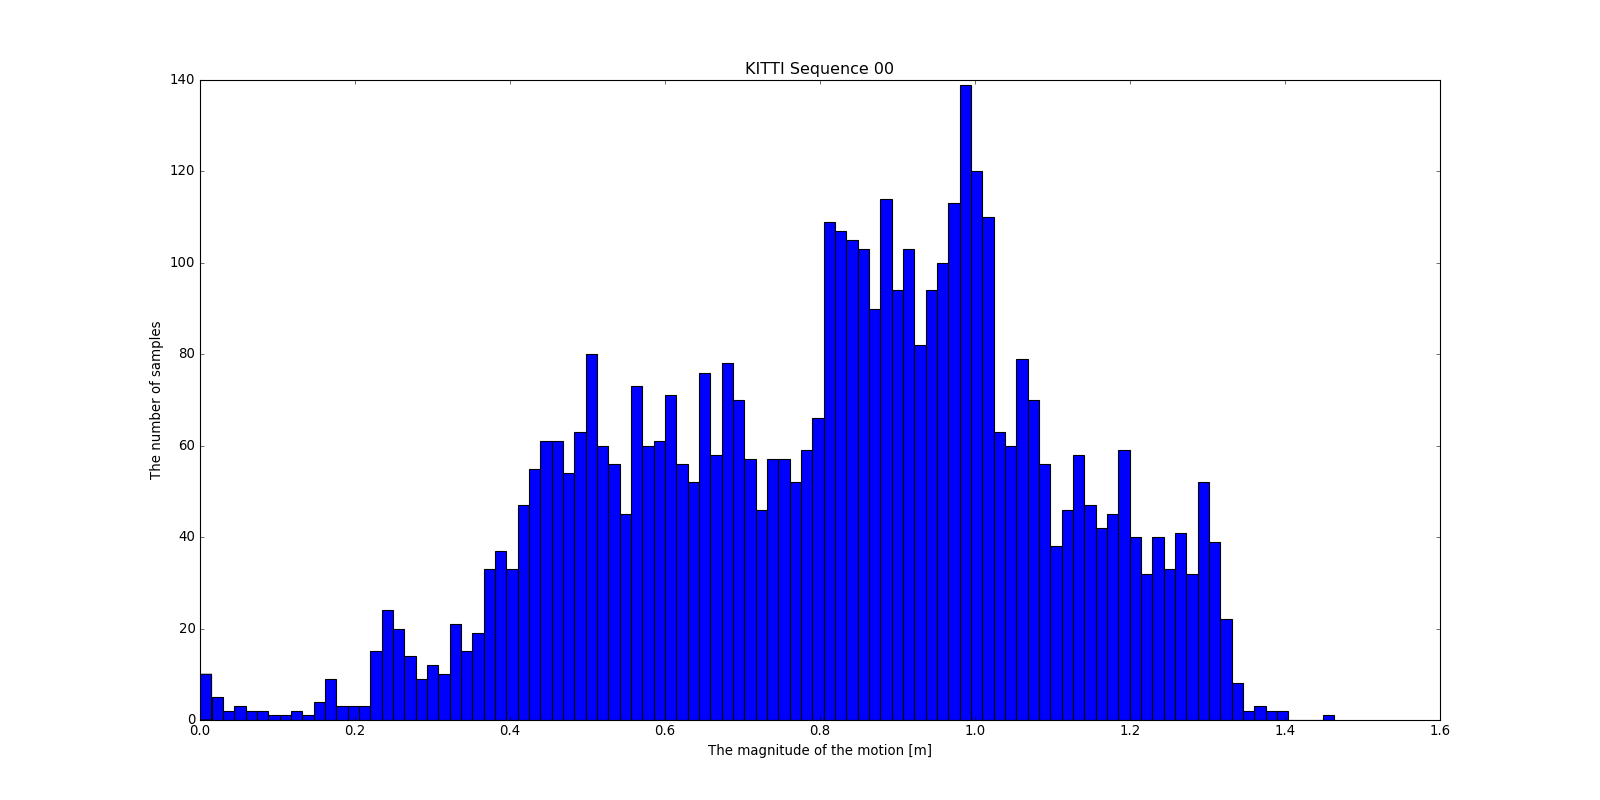
\includegraphics[width=4.5in]{00_t_distribution}
  \label{fig:t_distrib}
  \caption{The distribution of the camera translation magnitudes for the
    sequence '00'}
\end{figure}

\begin{figure}[ht]
  \hspace*{-4cm}
  \begin{subfigure}[b]{\linewidth}
    \centering
    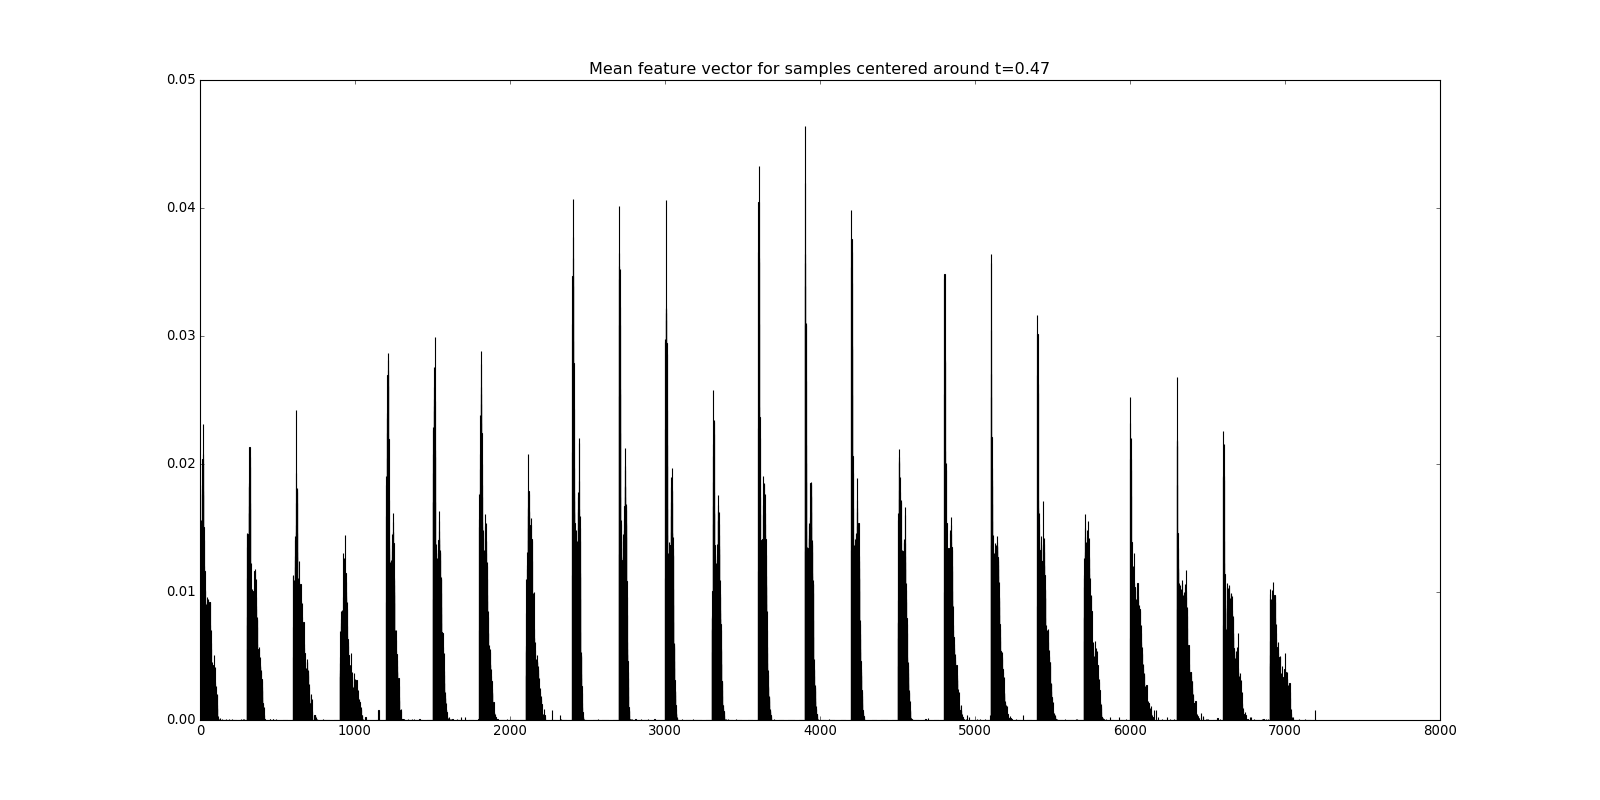
\includegraphics[width=4.0in]{00_mean_feature_vector_0_47}
    \caption{}\label{fig:1a}
  \end{subfigure}%
  \hspace*{-4cm}
  \begin{subfigure}[b]{\linewidth}
    \centering
    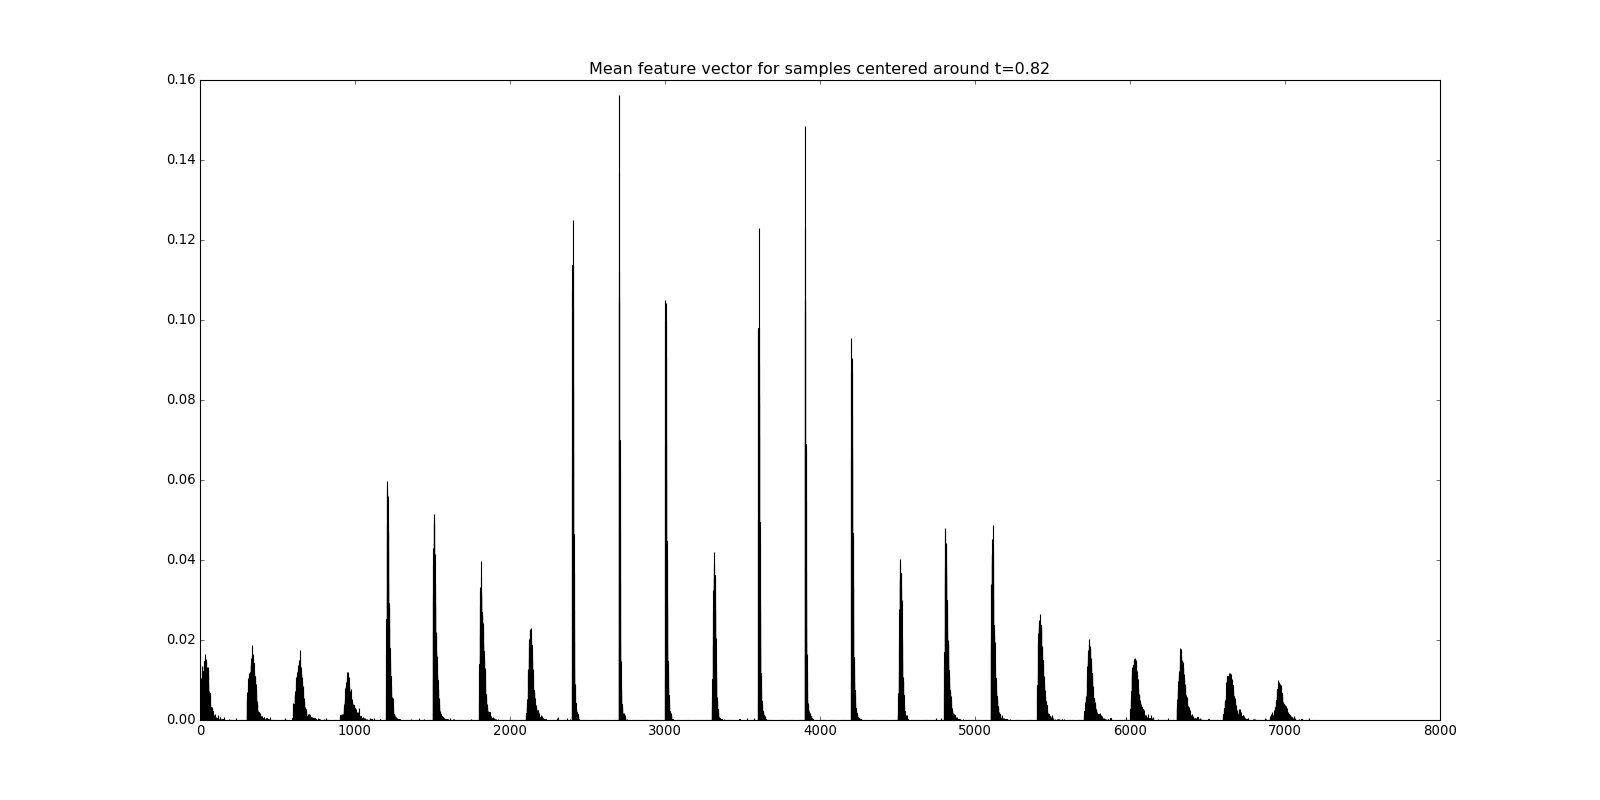
\includegraphics[width=4.0in]{00_mean_feature_vector_0_81}
    \caption{}\label{fig:1b}
  \end{subfigure}%
  \\
  \hspace*{-4cm}
  \begin{subfigure}[b]{\linewidth}
    \centering
    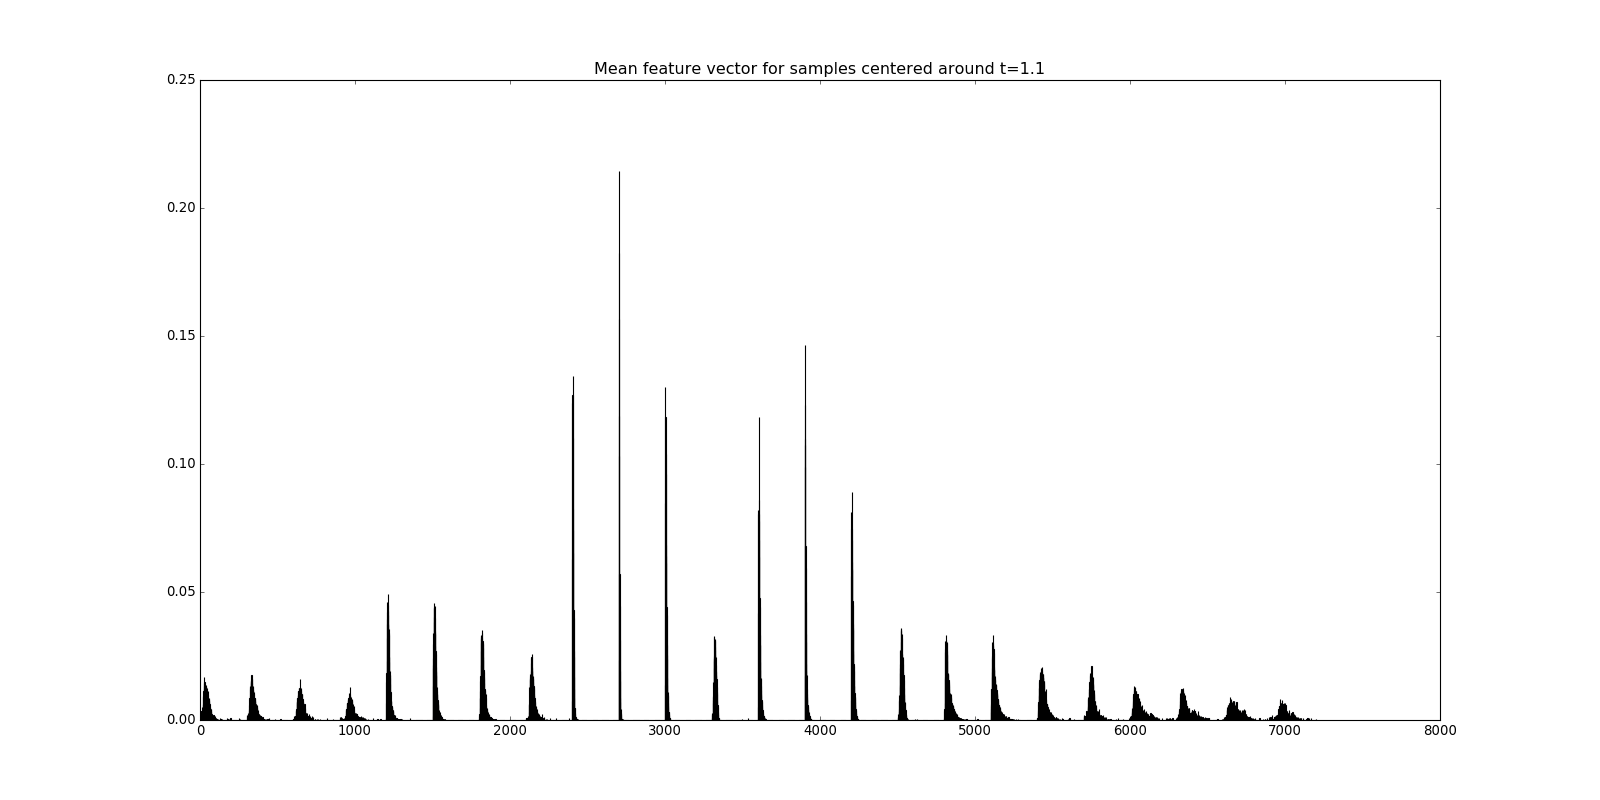
\includegraphics[width=4.0in]{00_mean_feature_vector_1_1}
    \caption{}\label{fig:1c}
  \end{subfigure}%
  \caption{Average feature vectors for samples centered around the
    specific camera translation magnitude.  Each peak corresponds to a
    grid cell (e.g. here the grid is 4 rows by 6 columns by 300 bins,
    so the feature vector is of the dimension 6*4*300=7200).  The grid
    is sampled in a column-major mode. So the first four peaks
    correspond to the leftmost column of the image grid.}
  \label{fig:feature_vectors}
\end{figure}

\section{Regression Models}

We train two different random forest models: the extremely random tree
forest (ERT) and the linear regression in the leafs ERT (LRERT).  The
difference is that the former averages the values in the leaf at test
time, while the latter fits a linear regression at each leaf, which is
used as a final predictor.  The implementation of the basic ERT is
taken from the sklearn library, while we implemented the the linear
regression in leafs features.

\section{Model Evaluation}

Figure~\ref{fig:1train_t_distrib} depicts the distribution of the
translation magnitudes in the training set. This training set was
produced by taking subsequent pairs of
images. Figure~\ref{fig:1model_eval} shows the model evaluation
results.


\emph{Note: ERT outperforms the linear regression in leafs ERT}.

\begin{figure}[ht]
  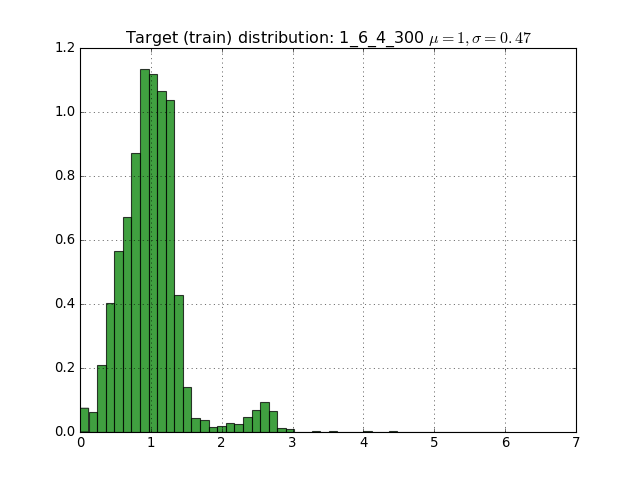
\includegraphics[width=4.0in]{1train_t_distribution}
  \caption{The distribution of the camera motion magnitudes for subsequent image pairs}
  \label{fig:1train_t_distrib}
\end{figure}

\begin{figure}[ht]
  \hspace*{-4cm}
  \begin{subfigure}[b]{\linewidth}
    \centering
    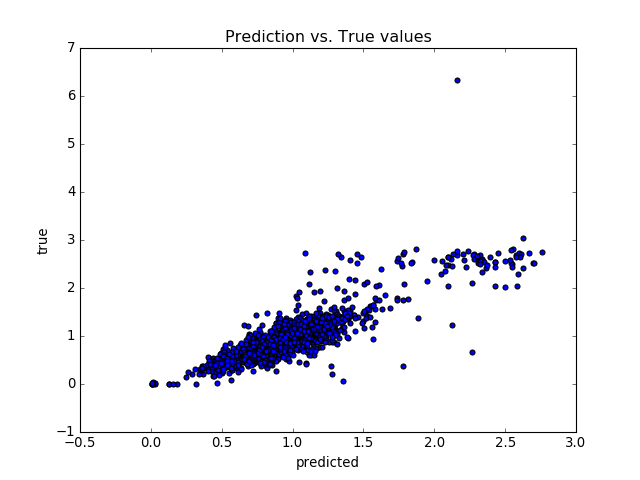
\includegraphics[width=3in]{1ERT_true_vs_predicted_RMSE_023}
    \caption{ERT: RMSE=0.23}\label{fig:2a}
  \end{subfigure}%
  \hspace*{-4cm}
  \begin{subfigure}[b]{\linewidth}
    \centering
    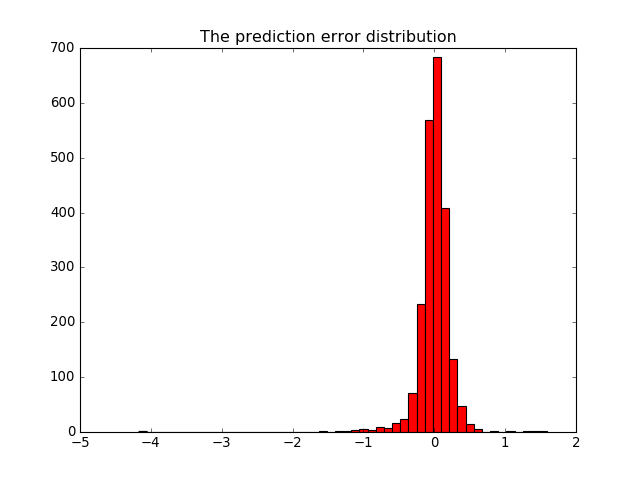
\includegraphics[width=3in]{1ERT_error_histogram_RMSE_023}
    \caption{ERT}\label{fig:2b}
  \end{subfigure}%
  \\
  \hspace*{-4cm}
  \begin{subfigure}[b]{\linewidth}
    \centering
    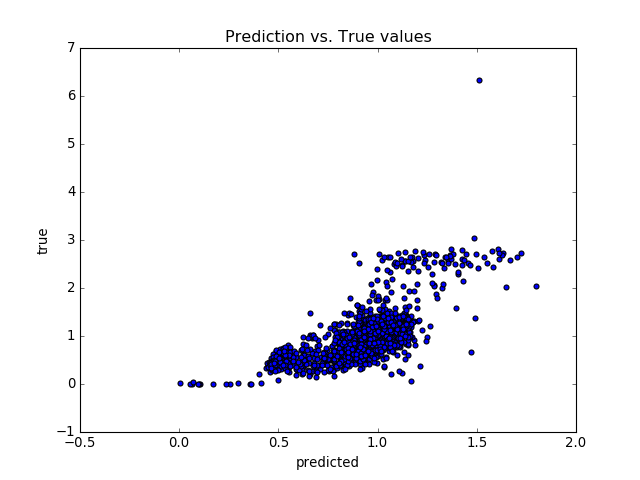
\includegraphics[width=3in]{1LRERT_true_vs_predicted_RMSE_036}
    \caption{LRERT: RMSE=0.36}\label{fig:2c}
  \end{subfigure}%
  \hspace*{-4cm}
  \begin{subfigure}[b]{\linewidth}
    \centering
    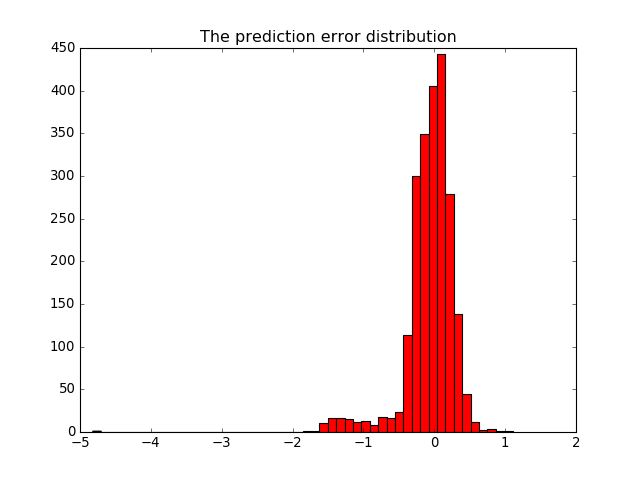
\includegraphics[width=3in]{1LRERT_error_histogram_RMSE_036}
    \caption{LRERT}\label{fig:2d}
  \end{subfigure}%
  
  \caption{Models evaluation over the validation set}
  \label{fig:1model_eval}
\end{figure}

\begin{figure}[ht]
  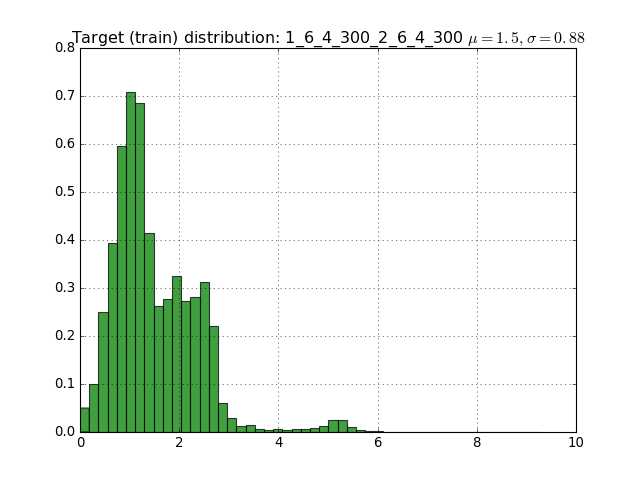
\includegraphics[width=4.0in]{12train_t_distribution}
  \caption{Dataset 2: contains the translation magnitudes for triplets of images (e.g. 2 subsequent camera motions)}\label{fig:2train_t_distrib}
\end{figure}

\begin{figure}[ht]
  \hspace*{-4cm}
  \begin{subfigure}[b]{.9\linewidth}
    \centering
    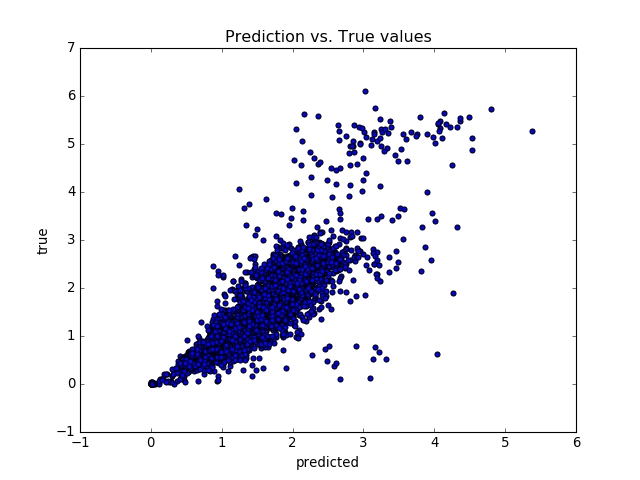
\includegraphics[width=3in]{12ERT_true_vs_predicted_RMSE_046}
    \caption{ERT: RMSE=0.46}\label{fig:3a}
  \end{subfigure}%
  \hspace*{-4cm}
  \begin{subfigure}[b]{.9\linewidth}
    \centering
    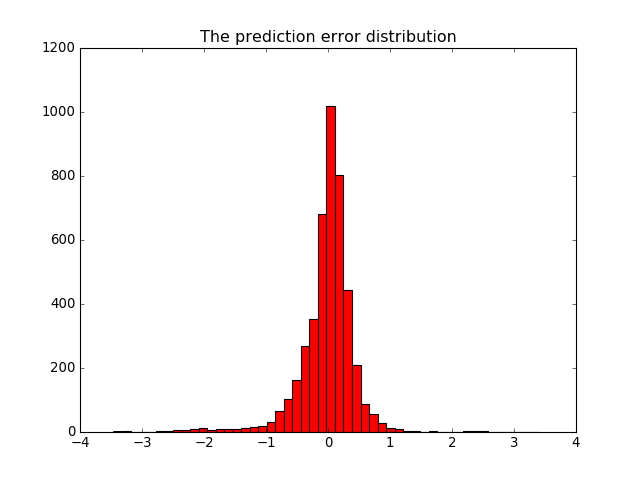
\includegraphics[width=3in]{12ERT_error_histogram_RMSE_046}
    \caption{ERT}\label{fig:3b}
  \end{subfigure}%
  \\
  \hspace*{-4cm}
  \begin{subfigure}[b]{.9\linewidth}
    \centering
    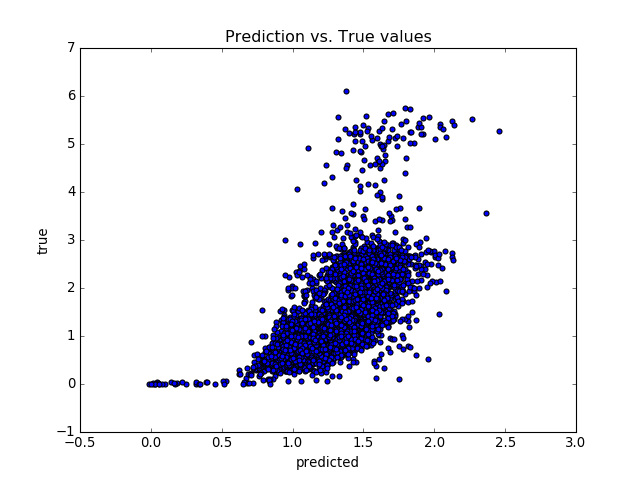
\includegraphics[width=3in]{12LRERT_true_vs_predicted_RMSE_075}
    \caption{LRERT: RMSE=0.75}\label{fig:3c}
  \end{subfigure}%
  \hspace*{-4cm}
  \begin{subfigure}[b]{\linewidth}
    \centering
    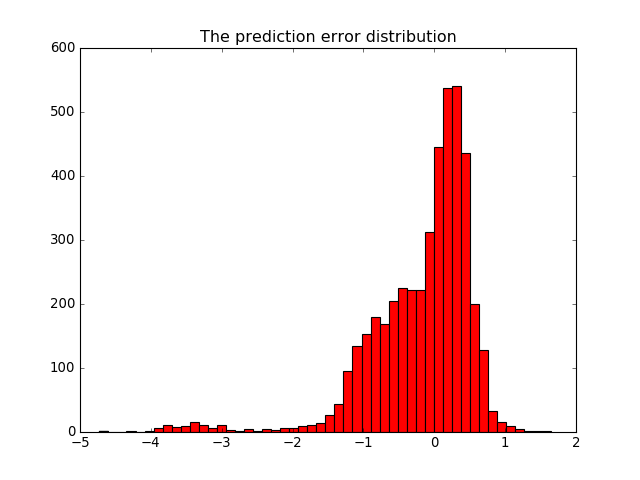
\includegraphics[width=3in]{12LRERT_error_histogram_RMSE_075}
    \caption{LRERT}\label{fig:3d}
  \end{subfigure}%
  
  \caption{Results for the dataset that contains image triplets}
  \label{fig:2model_eval}
\end{figure}

\section{Path Scale prediction}

Here we evaluate of the scenario where the monocular SLAM algorithm
produces a sequence of camera motion estimations which are correct up
to a single global scale (e.g. the relative scale of the subsequent
measurements is available).

Given a set of the relative translation magnitude measurements
(produced by the SLAM) $t_i$ and the set of the predicted (by the
trained models) scales $\hat{t}_i$ we search for the global scale $s_P$
s.t.

\[
  s_p = \underset{s}{\text{argmin}}\quad \sum_i{(st_i-\hat{t}_i)^2}
\]

The results of the path scale prediction are summarized in the Figure~\ref{fig:path_predict}
\begin{figure}[ht]
  \hspace*{-4cm}
  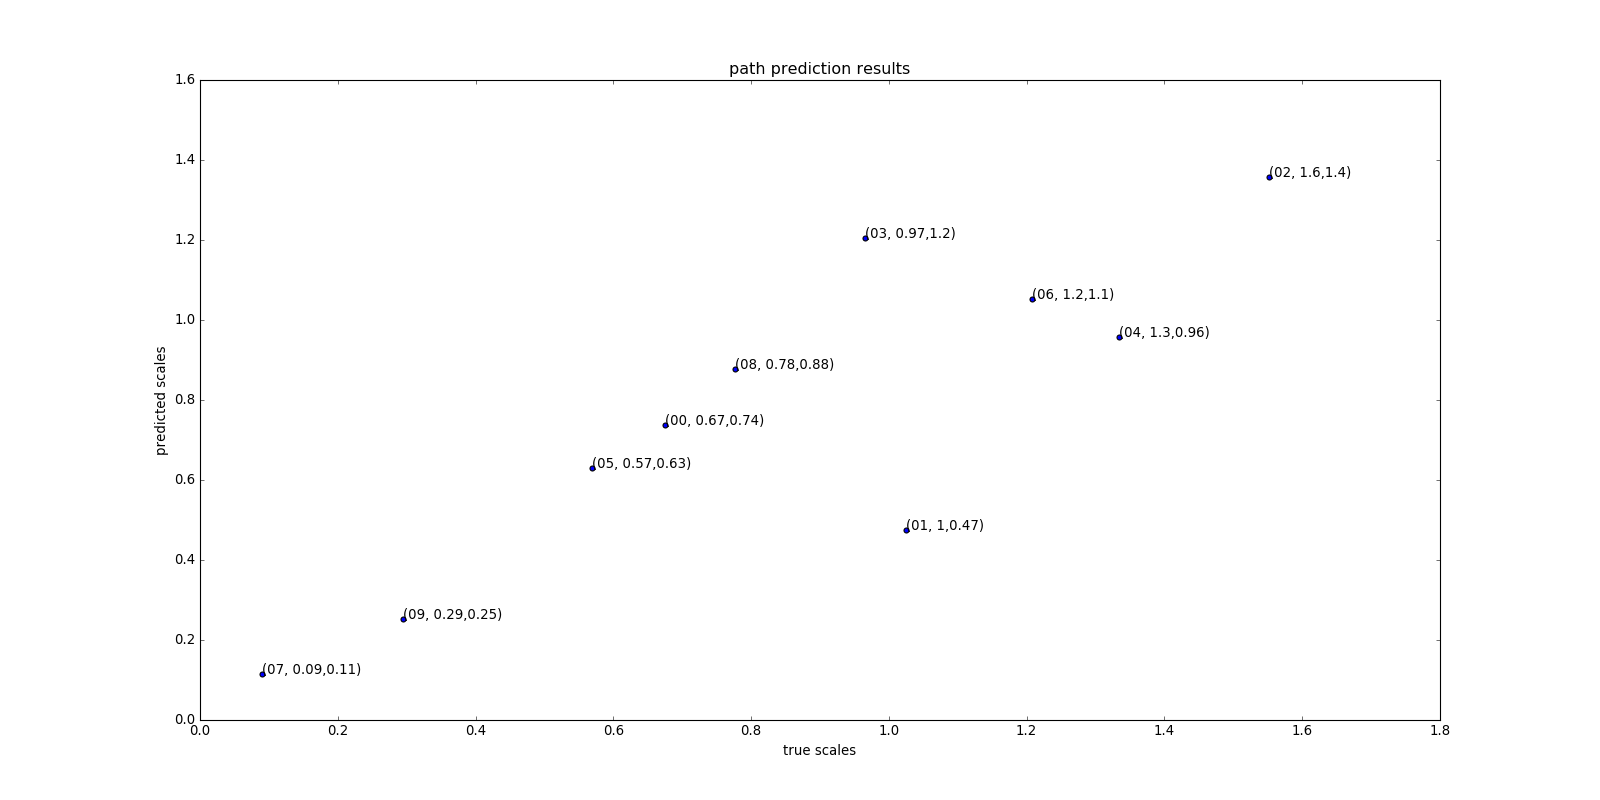
\includegraphics[width=7.5in]{path_predict}
  \caption{A path scale estimation results.  Each point is annotated with a triplet (KITTI sequence number, true scale, predicted scale)}\label{fig:path_predict}

\end{figure}

\end{document}

%%% Local Variables:
%%% mode: pdf
%%% TeX-master: t
%%% End:
